\section{Aufbau und Generierung der Irradiance Map} % (fold)
\label{sec:aufbau_und_generierung_der_irradiance_map}

	Im letzten Kapitel wurde die Irradianz $R$ der Szene $\Sigma$ nur an den Eckpunkten der Mesh evaluiert und gespeichert.
	Für Punkte im Inneren von Dreiecken führten wir eine lineare Interpolation durch.
	Die Approximation $\tilde{R}(x,\lambda)$ des Wertes $R(x,\lambda)$ für einen Punkt $x\in\e{T}$, der in einem Dreieck $(A,B,C)$ mit den baryzentrischen Koordinaten $(u,v,w)$ lag, und einer Wellenlänge $\lambda\in (0,\infty)$ beschrieben wir durch die folgende Definition.
	\[
		\tilde{R}(x,\lambda) \define w R(A,\lambda) + u R(B,\lambda) + v R(C,\lambda)
	\]
	Dieses Verfahren wird auch \enquote{Vertex Lighting} genannt und findet häufige Anwendungen in der Computerspieleindustrie \cite{tricks-game}.
	Vor allem bei der \enquote{Dragon}-Szene reichte diese Form der Intepolation aus, weil alle Dreiecke der Mesh klein genug waren, um den Verlauf der Irradianz gut zu beschreiben (siehe Abbildungen \ref{fig:irr-est-ra-dragon} und \ref{fig:irr-est-ra-dragon2}).
	Allerdings kam es bereits in der \enquote{Shaderball}-Szene zu ersten Interpolationsartefakten, wie in Abbildung \ref{fig:irr-est-ra-shaderball2} beim Übergang des Fußes in den Boden zu sehen ist.
	Solche Fehler treten immer dann auf, wenn zwischen zwei Eckpunkten eine unstetige oder extrem schnelle Änderung der Beleuchtung stattfindet.
	Ein typisches Beispiel dafür ist eine als Wand dienende Ebene, die die Szene teilt (siehe Abbildung \ref{fig:vertex-lighting-error}.

	\begin{figure}[h]
		\begin{subfigure}[t]{0.4\textwidth}
			\center
			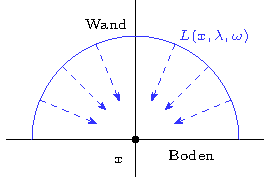
\includegraphics{gg_fig/vertex_lighting-error_1.pdf}
			\caption{Fehlerhafte Messung}
		\end{subfigure}
		\begin{subfigure}[t]{0.6\textwidth}
			\center
			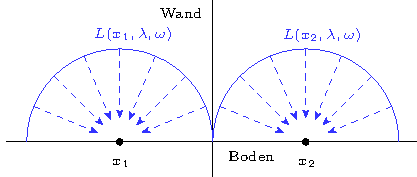
\includegraphics{gg_fig/vertex_lighting-error_2.pdf}
			\caption{Fehlerhafte Intepolation}
		\end{subfigure}
		\caption{Die Abbildung stellt die Ursachen der Fehler des Vertex Lighting dar. Fehler kann nur beseitigt werden, wenn die Punkte $x_1,x_2$ nah an der Wand, aber nicht auf der Wand gewählt werden.}
		\label{fig:vertex-lighting-error}
	\end{figure}

	Um Fehler dieser Art zu beheben, benötigen wir nicht nur Samplepunkte an den Eckpunkten der Dreiecke, sondern auch im Inneren dieser.
	Eine Variante die Anforderung zu erfüllen, besteht in der Verwendung von \enquote{Mesh Colors} \cite{mesh-colors}.
	Bei diesem Verfahren speichert man die aufgenommenen Werte an regelmäßigen Punkten des Dreiecks.
	Für jedes Dreieck gibt es dabei eine gewisse Freiheit in der Wahl der Anzahl von Samplepunkten.
	Abbildung \ref{fig:scheme-irr-map} zeigt dies genauer.

	\begin{figure}[h]
		\begin{subfigure}[t]{0.33\textwidth}
			\center
			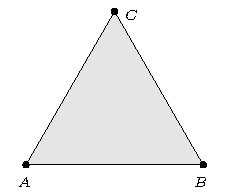
\includegraphics{gg_fig/irr_map_ds-order_1.pdf}
			\caption{\parbox[t]{0.5\textwidth}{Ordnung: $1$ \\ Samples: $3$}}
		\end{subfigure}
		\begin{subfigure}[t]{0.33\textwidth}
			\center
			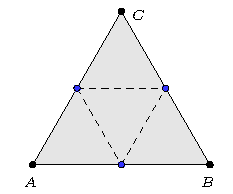
\includegraphics{gg_fig/irr_map_ds-order_2.pdf}
			\caption{\parbox[t]{0.5\textwidth}{Ordnung: $2$ \\ Samples: $6$}}
		\end{subfigure}
		\begin{subfigure}[t]{0.33\textwidth}
			\center
			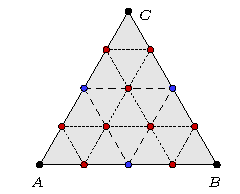
\includegraphics{gg_fig/irr_map_ds-order_4.pdf}
			\caption{\parbox[t]{0.5\textwidth}{Ordnung: $4$ \\ Samples: $15$}}
		\end{subfigure}
		\caption{Die Abbildung zeigt das Schema der Dreieck Irradianc Map Datenstruktur auf einem Dreieck $(A,B,C)$ für verschiedene Ordnungen.}
		\label{fig:scheme-irr-map}
	\end{figure}

	Die Anzahl der Samplepunkte für eine gegebene Ordnung $n\in\SN$ lässt sich durch die folgende Funktion beschreiben.
	\[
		\func{s}{\SN}{\SN},\qquad s(n)\define \frac{(n+1)(n+2)}{2}
	\]
	Beim Raytracing ist es üblich und meistens auch nötig die baryzentrischen Koordinaten des Schnittpunktes eines Strahls mit einem Dreieck zu berechnen \cite{ray-triangle-intersection}.
	Aus diesem Grund erscheint es sinnvoll jedem Samplepunkt einen zweidimensionalen Index zu geben, welcher ein besseres Auslesen ermöglichen wird.
	\[
		U_n\define \set[u+v\leq n]{(u,v)\in\SN_0^2},\qquad I_n\define \set[i < s(n)]{i\in\SN_0}
	\]
	\[
		\func{m_n}{U_n}{I_n},\qquad m_n(u,v) \define \frac{(u+v)(u+v+1)}{2} + v
	\]
	\[
		\func{m_{n,p}}{U_n}{I_{n\cdot 2^p}},\qquad m_{n,p}(u,v)\define m_{n\cdot 2^p}(u\cdot 2^p,v\cdot 2^p)
	\]
	In Abbildung \ref{fig:scheme-irr-map-memidx} sind die Definitionen der Indizierung für die Ordnungen $2$ und $4$ verdeutlicht.

	\begin{figure}[h]
		\begin{subfigure}[t]{0.5\textwidth}
			\center
			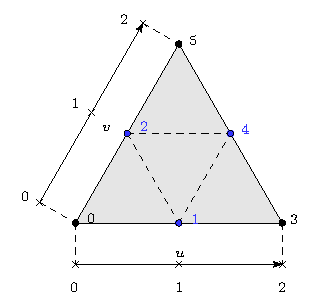
\includegraphics{gg_fig/irr_map_memidx-order_2.pdf}
			\caption{Ordnung: $2$}
		\end{subfigure}
		\begin{subfigure}[t]{0.5\textwidth}
			\center
			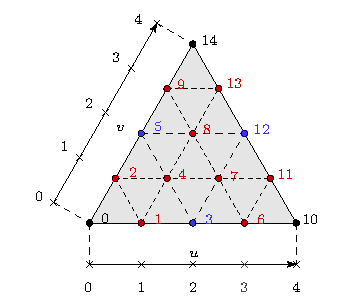
\includegraphics{gg_fig/irr_map_memidx-order_4.pdf}
			\caption{Ordnung: $4$}
		\end{subfigure}
		\caption{Die Abbildung zeigt das Schema der Dreieck Irradianc Map Datenstruktur für verschiedene Ordnungen.}
		\label{fig:scheme-irr-map-memidx}
	\end{figure}

	Der folgende Quelltext implementiert das Verfahren der Mesh Colors als Irradiance Map Datenstruktur für jedes Dreieck.
	\medskip
\begin{tcolorbox}[colframe=black,colbacktitle=white,coltitle=black, attach boxed title to top center={yshift=-2mm},enhanced, titlerule=0.1pt, boxrule=0.5pt, arc=5pt,title=Quelltext:\quad Dreieck Irradiance Map Datenstruktur, breakable]
	\lstinputlisting[style=std,language=c++]{code/irr_map.cpp}
\end{tcolorbox}
\medskip

	\medskip
\begin{tcolorbox}[colframe=black,colbacktitle=white,coltitle=black, attach boxed title to top center={yshift=-2mm},enhanced, titlerule=0.1pt, boxrule=0.5pt, arc=5pt,title=Quelltext:\quad Irradiance Map Generator, breakable]
	\lstinputlisting[style=std,language=c++]{code/gen_irr_map.cpp}
\end{tcolorbox}
\medskip

	\begin{figure}[h]
		\begin{subfigure}[b]{0.33\textwidth}
			\center
			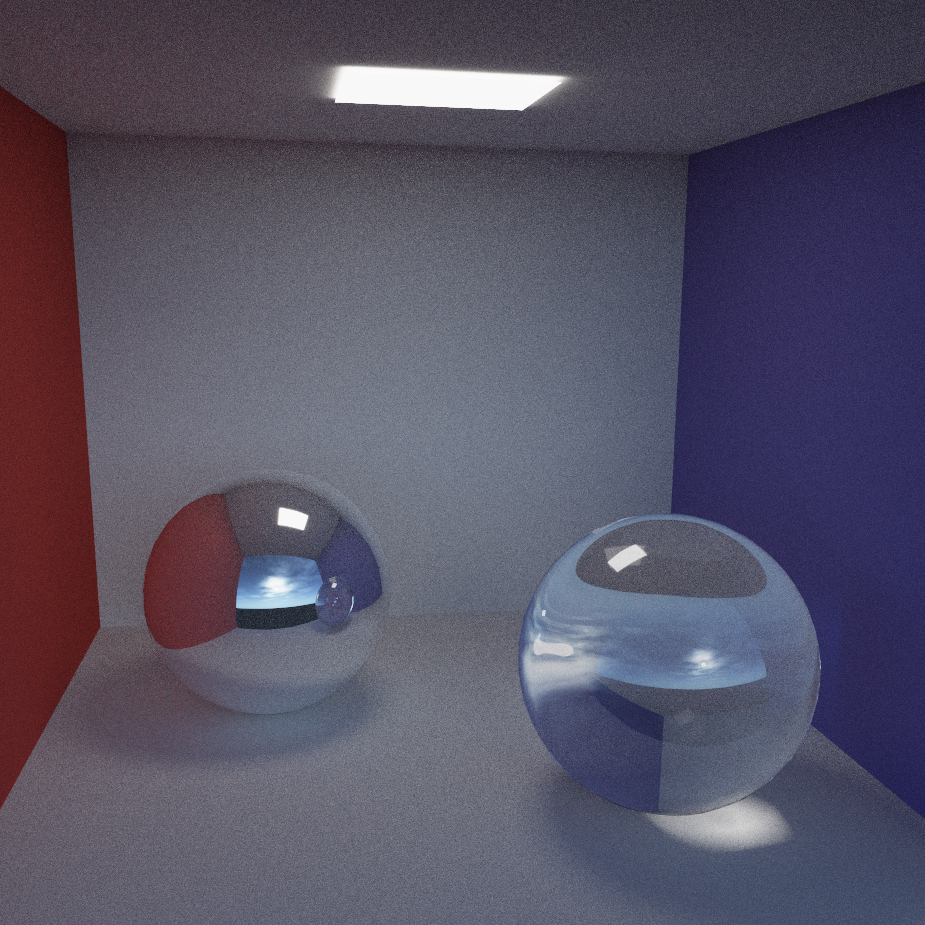
\includegraphics[width=0.95\textwidth]{pic/irrmap-cornell-ref.png}
			\caption{Path Tracing}
		\end{subfigure}
		\begin{subfigure}[b]{0.33\textwidth}
			\center
			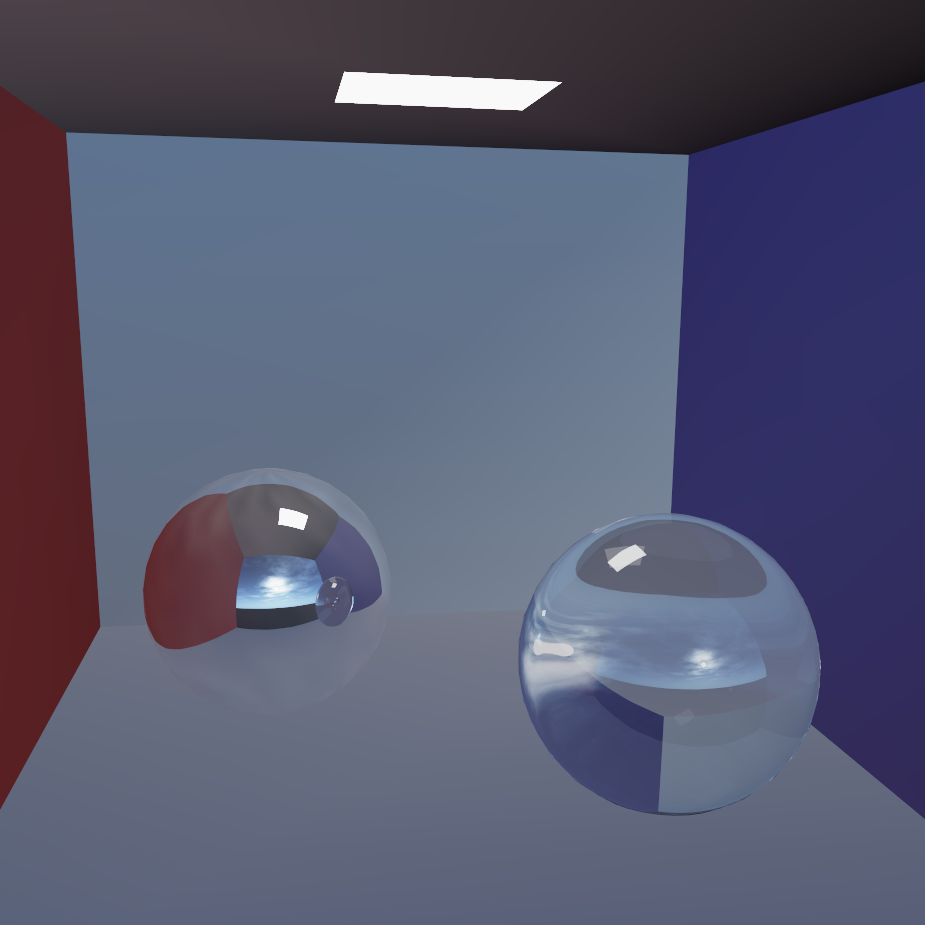
\includegraphics[width=0.95\textwidth]{pic/irrmap-cornell-vmap.png}
			\caption{Vertex Lighting}
		\end{subfigure}
		\begin{subfigure}[b]{0.33\textwidth}
			\center
			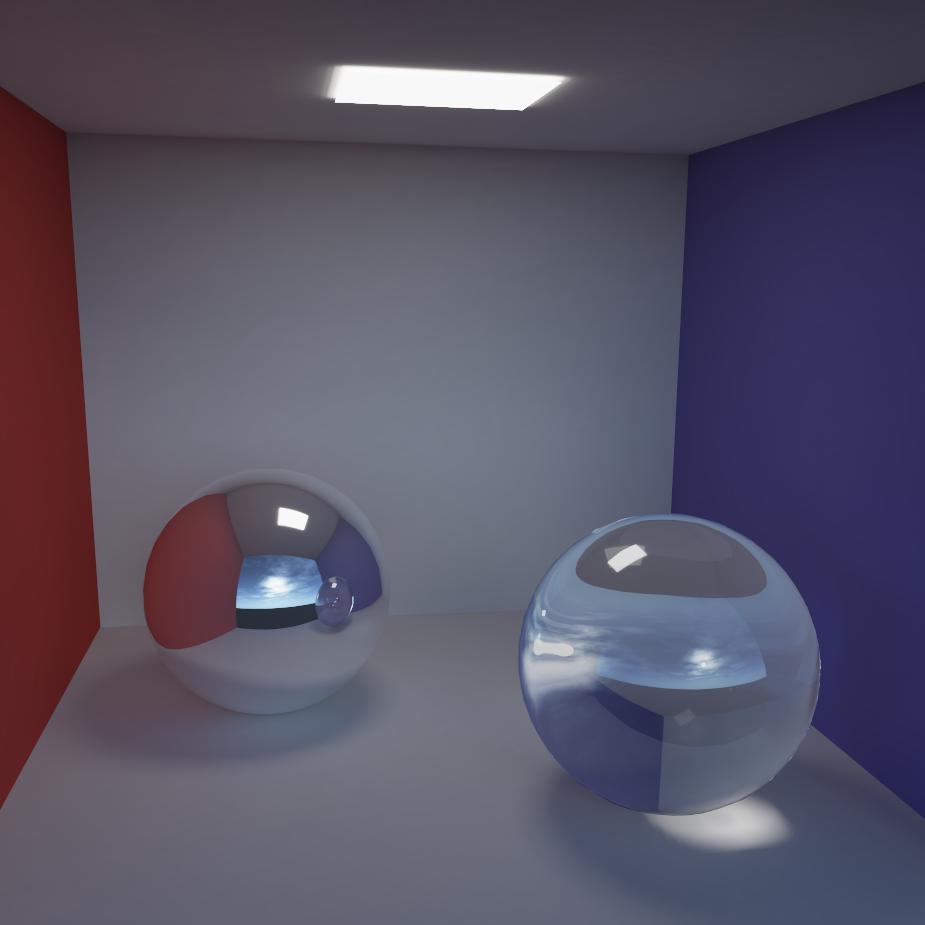
\includegraphics[width=0.95\textwidth]{pic/irrmap-cornell-irrmap.png}
			\caption{Irradiance Map}
		\end{subfigure}
		\caption[Irradiance-Map anhand der \enquote{Cornell Box}-Szene]{Die Bilder zeigen die Standardabweichungen der \enquote{Cornell Box}-Szene aus Abbildung \ref{fig:irr-est-rc-shaderball} entsprechend der Benennung aus Abbildung \ref{fig:irr-est-rc-dragon}. Vor allem Bereiche, die schwach von außen beleuchtet werden oder in Nischen liegen, weisen einen erhöhten Fehler auf. Die regelmäßigen Artefakte entstehen durch geringe Auflösung der Mesh in diesen Bereichen.}
		\label{fig:irr-map-cornell}
	\end{figure}

	\begin{figure}[h]
		\begin{subfigure}[b]{0.5\textwidth}
			\center
			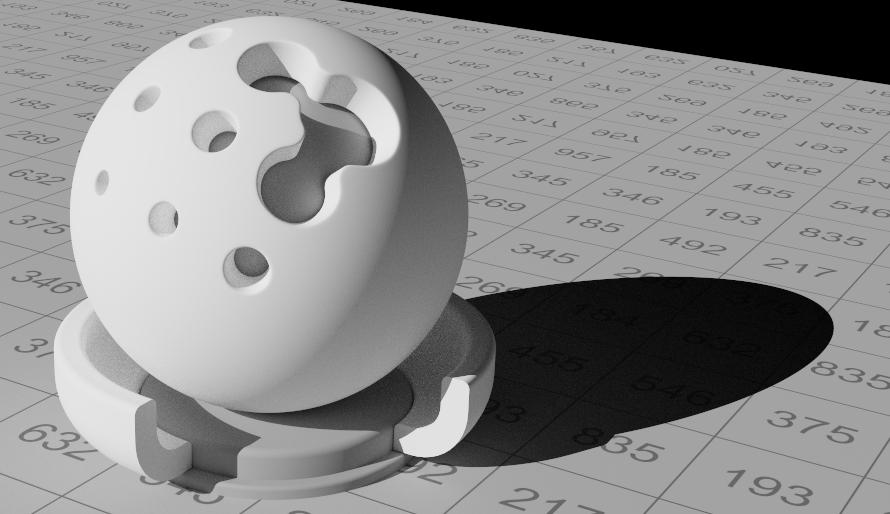
\includegraphics[width=0.95\textwidth]{pic/irrmap-shaderball-ref.png}
			\caption{Path Tracing}
		\end{subfigure}
		\begin{subfigure}[b]{0.5\textwidth}
			\center
			
\includegraphics[width=0.95\textwidth]{pic/irrmap-shaderball-vmap.png}
			\caption{Vertex Lighting}
		\end{subfigure}
		\smallskip \\
		\begin{subfigure}[b]{0.5\textwidth}
			\center
			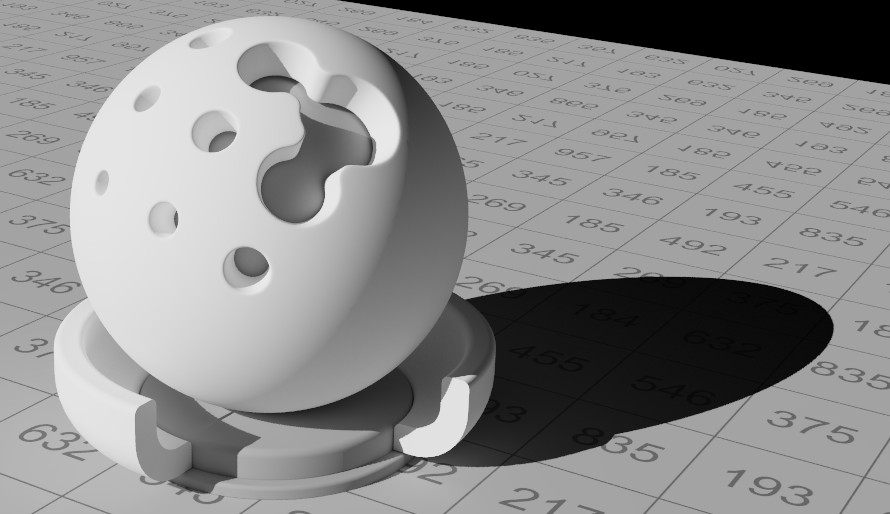
\includegraphics[width=0.95\textwidth]{pic/irrmap-shaderball-irrmap.png}
			\caption{Irradiance Map}
		\end{subfigure}
		\begin{subfigure}[b]{0.5\textwidth}
			\center
			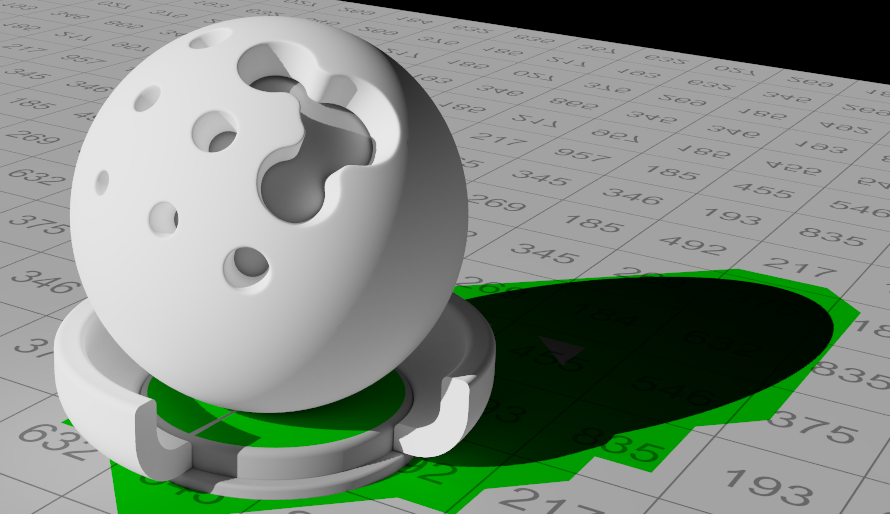
\includegraphics[width=0.95\textwidth]{pic/irrmap-shaderball-irrmap-order.png}
			\caption{Irradiance Map Ordnung}
		\end{subfigure}
		\caption[Irradiance-Map anhand der \enquote{Cornell Box}-Szene]{Die Bilder zeigen die Standardabweichungen der \enquote{Cornell Box}-Szene aus Abbildung \ref{fig:irr-est-rc-shaderball} entsprechend der Benennung aus Abbildung \ref{fig:irr-est-rc-dragon}. Vor allem Bereiche, die schwach von außen beleuchtet werden oder in Nischen liegen, weisen einen erhöhten Fehler auf. Die regelmäßigen Artefakte entstehen durch geringe Auflösung der Mesh in diesen Bereichen.}
		\label{fig:irr-map-cornell}
	\end{figure}

	\begin{figure}[h]
		\begin{subfigure}[b]{0.5\textwidth}
			\center
			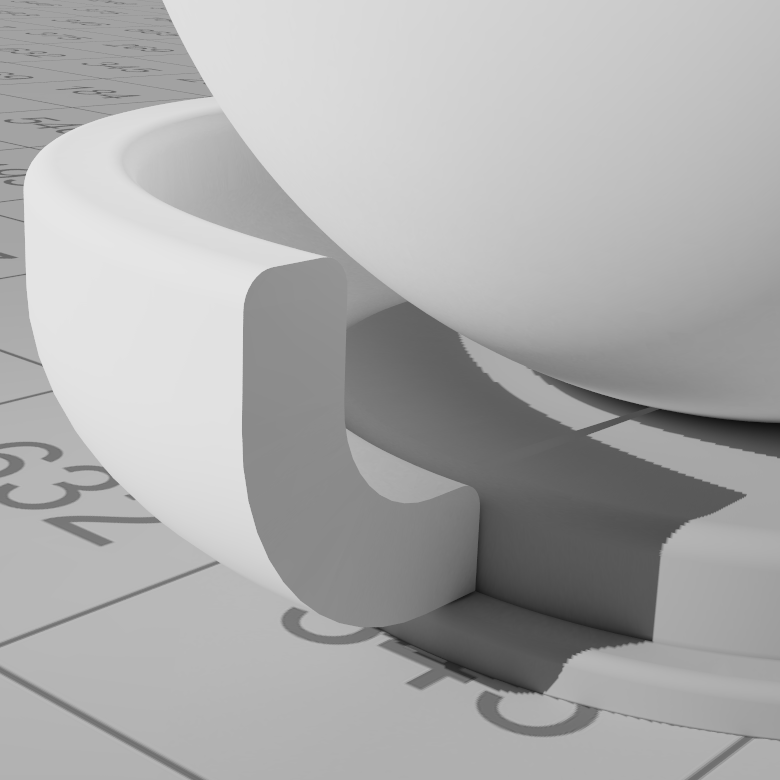
\includegraphics[width=0.95\textwidth]{pic/irrmap-shaderball2-irrmap.png}
			\caption{Irradiance Map}
		\end{subfigure}
		\begin{subfigure}[b]{0.5\textwidth}
			\center
			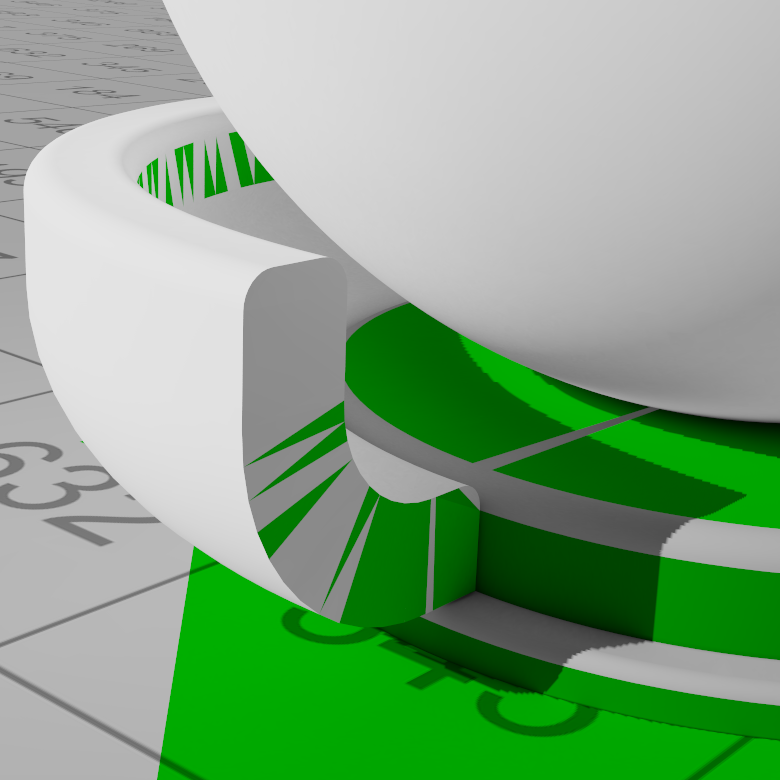
\includegraphics[width=0.95\textwidth]{pic/irrmap-shaderball2-irrmap-order.png}
			\caption{Irradiance Map Ordnung}
		\end{subfigure}
		\caption[Irradiance-Map anhand der \enquote{Cornell Box}-Szene]{Die Bilder zeigen die Standardabweichungen der \enquote{Cornell Box}-Szene aus Abbildung \ref{fig:irr-est-rc-shaderball} entsprechend der Benennung aus Abbildung \ref{fig:irr-est-rc-dragon}. Vor allem Bereiche, die schwach von außen beleuchtet werden oder in Nischen liegen, weisen einen erhöhten Fehler auf. Die regelmäßigen Artefakte entstehen durch geringe Auflösung der Mesh in diesen Bereichen.}
		\label{fig:irr-map-cornell}
	\end{figure}

% section aufbau_und_generierung_der_irradiance_map (end)